\chapter{Refactoring}
\section{Code Smell 1 - Lange Methode}
Der erste Code Smell, der identifiziert wurde, ist langer übersichtlicher Code, der dafür genutzt wurde, um Transaktionen in einer Mail aufzulisten und an den eingeloggten Benutzer zu versenden. 
Diese Methode ist die \glqq getTransactionsAsMail \grqq -Methode, die sich in der \glqq TransactionRepositoryImpl \grqq -Klasse befindet.
In dieser Methode werden zum einen alle Transaktionen für ein Konto abgerufen und zum anderen ein Mail-Objekt aufgrund der abgefragten Transaktionen erstellt. Es wurde, um die Übersichtlichkeit zu 
verbessern, die Funktion, die das Mail-Objekt erstellt, in eine neue Methode extrahiert. In \ref{codeSmell1} ist die unübersichtliche Methode zu sehen. In \ref{codeSmell1Nachher} ist die Methode zu sehen nach dem Refactoring.
\begin{figure}[htbp]
    \centering
    \fbox{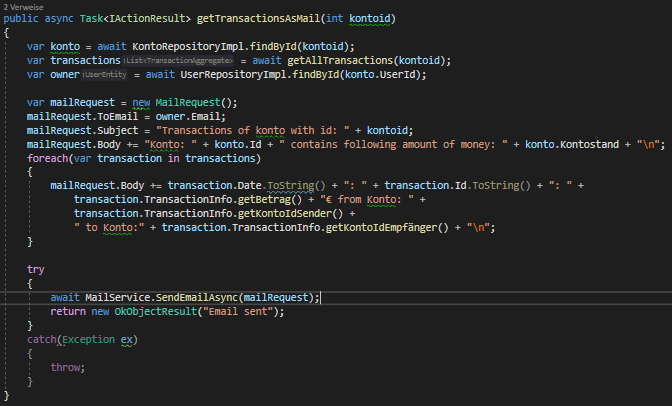
\includegraphics[width=10cm]{CodeSmell1Vorher.png}}
    \caption{\label{codeSmell1} Long Method}
\end{figure}
\begin{figure}[htbp]
    \centering
    \fbox{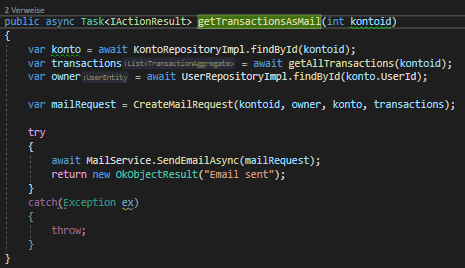
\includegraphics[width=10cm]{CodeSmell1Nachher.png}}
    \caption{\label{codeSmell1Nachher} Long Method Refactored}
\end{figure}
\section{Code Smell 2 - Duplikate im Code}
Der zweite Code Smell, der identifiziert wurde, ist ein Duplikat im Code. Es wurde zwar versucht nach dem DRY-Prinzip zu arbeiten, dies wurde jedoch nicht hundertprozentig umgesetzt. Später lies sich beispielsweise in der \glqq UserController \grqq -Klasse 
ein Duplikat finden, in welchem eine Liste an UserEntities in eine Liste von User-Objekten durch einen den Mapper konvertiert wurde. Diese Funktion wurde in mehreren Methoden dieser Klasse verwendet. 
\newline Um das Duplikat zu verhindern, wurde diese Funktion in eine neue Methode innerhalb des Mappers ausgelagert, durch welche nun eine Liste an UserEntities in eine Liste an User-Objekten umgewandelt wird. 
Diese Methode wird von mehreren Stellen aufgerufen. In \ref{codeSmell2Vorher} wird der Code, der dupliziert vorkam, in einer der Methoden gezeigt.
\begin{figure}[htbp]
    \centering
    \fbox{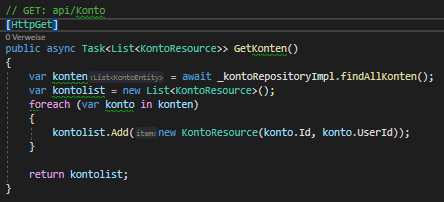
\includegraphics[width=10cm]{CodeSmell2Vorher.png}}
    \caption{\label{codeSmell2Vorher} Duplicate Code}
\end{figure}
\begin{figure}[htbp]
    \centering
    \fbox{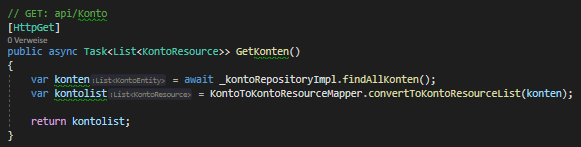
\includegraphics[width=10cm]{CodeSmell2Nachher.png}}
    \caption{\label{codeSmell2Nachher} Duplicate Code Refactored}
\end{figure}
In \ref{codeSmell2Nachher} wird gezeigt, wie die Funktion ausgelagert wurde und durch den Mapper aufgerufen wird. Diese Funktion wird noch an weiteren Stellen innerhalb des Controllers aufgerufen.